%%% start preambling . . .  %%%
\documentclass[12pt]{article}
% \setmainfont{Times New Roman}
% required 

% EMW recommends parskip now instead of \\ too much: https://www.overleaf.com/learn/latex/Articles/How_to_change_paragraph_spacing_in_LaTeX#The_parskip_package ... add \usepackage{parskip} to preamble, delete \\ and see how it looks
\UseRawInputEncoding % helps with "LaTeX Error: Invalid UTF-8 byte sequence"
\usepackage{parskip}
\usepackage{amsmath}
\usepackage[T1]{fontenc}
% \usepackage[natbibapa]{apacite}  % this is apa
% \bibliographystyle{apacite} % this is apa
\usepackage[comma]{natbib}
\bibliographystyle{agsm} %Harvard referencing style
\usepackage{xr-hyper}
\usepackage{hyperref}
\externaldocument[supplement-]{supplement}
\usepackage{booktabs,siunitx}
\usepackage{Sweave}
\usepackage{xurl}
\usepackage{graphicx}
\usepackage{lipsum}                     % Dummytext % https://tex.stackexchange.com/questions/9796/how-to-add-todo-notes
\usepackage{xargs}                      % Use more than one optional parameter in a new commands
\usepackage[pdftex,dvipsnames]{xcolor}  % Coloured text etc.
\usepackage[colorinlistoftodos,prependcaption,textsize=tiny]{todonotes}
\newcommandx{\unsure}[2][1=]{\todo[linecolor=red,backgroundcolor=red!25,bordercolor=red,#1]{#2}}
\newcommandx{\change}[2][1=]{\todo[linecolor=blue,backgroundcolor=blue!25,bordercolor=blue,#1]{#2}}
\newcommandx{\info}[2][1=]{\todo[linecolor=OliveGreen,backgroundcolor=OliveGreen!25,bordercolor=OliveGreen,#1]{#2}}
\newcommandx{\improvement}[2][1=]{\todo[linecolor=Plum,backgroundcolor=Plum!25,bordercolor=Plum,#1]{#2}}
\newcommandx{\thiswillnotshow}[2][1=]{\todo[disable,#1]{#2}}
% https://tex.stackexchange.com/questions/60209/how-to-add-an-extra-level-of-sections-with-headings-below-subsubsection
\usepackage{titlesec}
\setcounter{secnumdepth}{4}

\titleformat{\paragraph}
{\normalfont\normalsize\bfseries}{\theparagraph}{1em}{}
\titlespacing*{\paragraph}
{0pt}{3.25ex plus 1ex minus .2ex}{1.5ex plus .2ex}

% recommended! Uncomment the below line and change the path for your computer!
 
%put your figures in one place! Also, note that here 'figures' is the folder and 'demoFig' is what each 
% figure produced will be titled plus its number or label (e.g., demoFig-nqpbetter.pdf')
% make your captioning look better
\usepackage[small]{caption}
\setlength{\captionmargin}{30pt}
\setlength{\abovecaptionskip}{0pt}
\setlength{\belowcaptionskip}{10pt}
% optional: muck with spacing
\topmargin -1.5cm        
\oddsidemargin 0.5cm   
\evensidemargin 0.5cm  % same as oddsidemargin but for left-hand pages
\textwidth 15.59cm
\textheight 21.94cm 
% \renewcommand{\baselinestretch}{1.5} % 1.5 lines between lines
\parindent 0pt		  % sets leading space for paragraphs
% optional: cute, fancy headers
\usepackage{fancyhdr}
\pagestyle{fancy}
\fancyhead[LO]{2024}
\fancyhead[RO]{Manuscript}
\usepackage{lineno} %alinaSep22: this is to number each line (GCB requires it). However, I dont know how not to number the title page, and I also would like the number to appear bigger. Can lizzie fix this please?
\usepackage{setspace}
% Using \doublespacing in the preamble changes the text to double-line spacing
% \doublespacing
\setstretch{1.5} %1.5 spacing
% more optionals! %
% \usepackage[hyphens]{url} % this wraps my URL versus letting it spill across the page, a bad habit LaTeX has
%%% end preambling. %%%

\begin{document}
\Sconcordance{concordance:supplement.tex:supplement.Rnw:%
1 65 1}
 % For RStudio hiccups
\begin{flushright}
Version dated: \today
\end{flushright}

\bigskip
\medskip
\begin{center}

% Insert your title:
\noindent{\Large {\bf Weak evidence of provenance effects in spring phenology across Europe and North America}}\\ 
\bigskip

\noindent {\normalsize \sc
Z. A. Zeng $^{1}$ \& E. M. Wolkovich$^{2}$}\\


\noindent {\small \it
$^1$ Forest Resources Management, Faculty of Forestry, University of British Columbia, 2424 Main Mall, Vancouver, BC V6T 1Z4\\
$^2$ Forest \& Conservation Sciences, Faculty of Forestry, University of British Columbia, 2424 Main Mall, Vancouver, BC V6T 1Z4}
\end{center}
\medskip
\noindent{\bf Corresponding author:} Z. A. Zeng, see $^{1}$ above ; E-mail: alinazengziyun@yahoo.com\\
\noindent{\bf Additional information:} Zeng (0009-0000-4647-9457); Wolkovich (0000-0001-7653-893X)\\
\noindent{\bf Running head:} Clines in spring phenology\\
\noindent{\bf Word count:} Summary - 198, Introduction - 1077, Materials and Methods - 821, Results - 1012, Discussion - 1400\\
\noindent{\bf Number of figures:} 4 (Among these, Figure 1 and 2 should be published in color)\\
1. Figure 1: Map showing the distribution of common gardens and provenances.\\
2. Figure 2: Event day of year in relation to provenance latitude and MAT.\\
3. Figure 3: Effects of latitude on spring and fall event day of year depending on continent and species leaf type.\\
4. Figure 4: Effects of MAT on spring and fall event day of year depending on continent and species leaf type.\\
\noindent{\bf Supporting Information (brief legends):}\\
1. Methods S1: Additional methods.\\
2. Table S1: Showing all publications included in meta-analysis.\\
3. Table S2-5: Showing summary of model estimates.\\
4. Figures S1-3: Supporting figures.


\newpage
% Journal ideas: Global Change Biology; Functional Ecology or Journal of Ecology next seem good ... maybe a biogeography journal (though I am not sure if we can afford one) ... maybe New Phytologist but I think they could be picky. 
\linenumbers

\section*{Summary}

% \begin{abstract} %EWMFeb5 -- edited to define provenance differences 

\begin{itemize} %EMWFeb20 -- small tweaks to improve flow and we do not need to say 'population' so much, methinks. 
  \item Forecasting the biological impacts of climate change requires understanding how species respond to warmer temperatures through inter-annual flexible variation vs. through adaptation to local conditions. Yet, we often lack this information entirely or find conflicting evidence across studies, which is the case for spring phenology.
  \item We synthesize common garden studies across Europe and North America that reported spring event dates for a mix of angiosperm and gymnosperm tree species in the northern hemisphere, capturing data from 384 North American and 101 European provenances (i.e. populations) with observations from 1962 to 2019, alongside fall event data when provided.
  \item Across continents, we find no evidence of provenance effects in spring phenology, but strong clines with latitude and mean annual temperature (MAT) in fall. These effects, however, appear to diverge by continent and species type (gymnosperm vs. angiosperm), with particularly pronounced clines in North America in fall events.
  %EWMFeb5 -- if you need to save words, can cut 'due to provenance effects' below. 
  \item Our results suggest flexible, likely plastic responses, in spring phenology with warming, and potential limits---at least in the short term---due to provenance effects for fall phenology. They also highlight that, after over 250 years of common garden studies on tree phenology, we still lack a holistic predictive model of clines across species and phenological events.
\end{itemize}
% Forecasting the biological impacts of climate change requires understanding how species respond to warmer temperatures through inter-annual flexible variation versus through adaptation to local conditions. Yet, we often lack this information entirely or find conflicting evidence across studies. The latter is the case for shifts in spring phenology---one of the most reported and consistent impacts of anthropogenic climate change, and also one of the most critical to forecasting, given its role in carbon sequestration. Some common garden studies have found evidence of important provenance effects (i.e. population differences), which suggest there may be local adaptation in the underlying cues of spring phenology and mirrors findings for fall events, while other studies find no evidence. Here, we synthesize common garden studies across Europe and North America that reported spring event dates for a mix of angiosperm and gymnosperm tree species in the northern hemisphere, capturing data from 384 North American provenances and 101 European provenances with observations from 1962 to 2019, alongside fall event data when provided. Across continents, we find no evidence of provenance effects in spring phenology, but strong clines with latitude and mean annual temperature (MAT) for fall events. These effects, however, appear to diverge by continent and species type (gymnosperm versus angiosperm), especially for fall events where clines with latitude and MAT are much stronger in North America. Our results suggest flexible, likely plastic responses, in spring phenology with warming, and potential limits---at least in the short term---due to provenance effects for fall phenology. They also highlight that, after over 250 years of common garden studies on tree phenology, we still lack a holistic predictive model of clines across species and phenological events. 
% \end{abstract} 

\noindent \emph{Keywords: budburst, budset, climate change, common gardens, deciduous and evergreen trees, leafout, senescence, spring phenology}\\ %EWMFeb5 -- if you have an abundance of keywords, remove ones that are redundant with title/abstract


\section{Introduction}

%emw: I noticed a lot of papers on local adaptation don't always use the term 'local adaptation' so we may want to avoid using it too much? I suspect it may be contested. I also wonder if my advice about definitions was wrong ... but let's definitely save that text for now. 
%emw: We need to 'funnel' in our intros -- until we submit to a plant journal focusing on plants too early is getting too narrow too fast. 

% To optimize ecosystem services for habitat conservation and understand how plants cope with environmental variations, predicting the biological impacts of climate change is of critical importance \citep{botero15}. One of the most important parts of accurate prediction is understanding the relative importance of local adaptation versus plasticity \citep{chevin10}. 
Predicting the biological impacts of climate change has made understanding how organisms cope with environmental variation more urgent \citep{botero15}. In particular, the relative importance of plasticity versus genetic adaptation is vital for prediction \citep{chevin10}, with plasticity expected to allow species to shift more rapidly with climate change than environmental responses based on local adaptation, but possibly stalling responses after the limits of plasticity are reached \citep{chevin102,snell18}.

% Local adaptation---how well the growth and adaptive characteristics align with the local climate conditions---influences their ability to thrive and reproduce  \citep{casmey22, kawecki04, anderson12, kim13}. When the selection intensity exceeds gene flow in species that spread over diverse areas, clinal variations among environmental factors can result in populations with unique adaptations to the local climate and, therefore, greater fitness \citep{kremer12, rossi15, salmela13}. On the other hand, phenotypic plasticity describes an individual genotype’s ability to exhibit different phenotypes in response to environmental variations, enabling plants to adjust to new environmental conditions and survive in this rapidly changing world (also known as `plastic rescue')  \citep{chevin10, chevin102, snell18}. 

% emwJun4: I really love the info you added here, but we have to be careful to not focus too deeply on synchrony as it is a very specific topic and our work is broader than that (sorry if I confused you by my request for 'refs' -- I mostly wanted just citations; I suspect we can use some of the text for the discussion so it will not go to waste). We also need to keep paragraphs themselves and our intro overall short, so I cut here. Thus I slimmed this way down and kept many references, but less of the examples.
Many of the currently observed responses to climate change appear to be mainly plastic \citep{burton22,zettle21,bonamour19, king17}, including the most reported biological response to climate change---shifting phenology. Phenology---the timing of recurring seasonal events---governs the timing of transitions between dormancy and active growth for many organisms, allowing them to time reproduction and exploit the resources of each growing season \citep{chuine10,hanninen11,rytteri21,posle18}. As such, phenology plays a significant role in determining fitness for both plants \citep{guo22,chuine01} and animals \citep{wann19,renner18,chu17}. 

Shifted phenology in recent decades---with many events moving several days per decade \citep{vita21,khar18,Menzel06}---has led to concerns about fitness consequences, and the limits of possible future shifts. While future phenological shifts will depend on how much phenology is determined by plasticity versus adaptation, our understanding of the balance of these two approaches to variation is limited. This is the case even for species groups that are critical to both forecasting and have been well studied, such as trees. 

Tree phenology is important to climate change forecasting at both the community and ecosystem levels. The timing of budburst and senescence can impact plant competition, plant invasions, and community assembly \citep{fridley12}. Shifts in phenology can affect tree growth \citep{myneni97}, scaling up to impact ecosystem-level carbon sequestration \citep{Barichivich12}, and thus forecasts of climate change. Growing evidence, however, suggests links between growth and phenology are not as consistent as previously predicted---or currently modelled \citep{dow22}---with recent work suggesting how much spring versus fall events shift may determine impacts on tree growth \citep{zohner23}. 

%EWMFeb5 -- edits below to define provenance; and added a reference to 'local adaptation'
Studies of adaptation versus plasticity in tree phenology have been conducted for centuries \citep{Cleland:2007or}, through common garden studies. In these studies---conducted often for forestry purposes---researchers grow trees of different geographical origins (called `provenances' often in forestry) under the same environmental conditions to disentangle the effects of environmental and genetic variation on trees' phenotypes \citep{AitkenBemmels16, Alberto13}. Such work has established common clines in fall phenology suggestive of local adaptation, as source locations with shorter growing seasons (poleward and higher elevations) exhibit earlier growth cessation (such as budset). Research has connected these clines to an underlying proximate mechanism of changing photoperiod cues (i.e., shifts in the photoperiod threshold required to trigger budset), driven by adaptation to the local growing season \citep{Alberto13,Savolainen07}. In contrast, spring phenology appears more plastic \citep{AitkenBemmels16} and determined more strongly by temperature \citep{flynn18}. Many studies, however, have argued that spring phenology shows levels of adaptation that may be critical to forecasting and mitigation \citep{vitasse2009,Basler:2012}. 

These contrasting studies highlight how inconsistent evidence for adaptation in tree spring phenology has been. Studies have documented provenance differences of 2-4 days per degree latitude in spring phenology for some species (\emph{Picea abies} in \citealp{sog08} and \emph{Quercus petraea} in \citealp{deans96}) while others have failed to find similar trends along latitudinal gradients (for example, \emph{Picea sitchensis} in \citealp{mimura07}, \emph{Picea glauca} in \citealp{Li97}, and \emph{Populus balsamifera} in \citealp{farmer93}). This has led to debate over the prevalence and importance of adaptation in spring tree phenology. Though clines of spring phenology have been found in both Europe \citep{sog08,deans96,von95} and North America \citep{rossi15, soo13, hannerz99}, there is continuing debate, especially in Europe \citep{deans96,vitasse2009,Basler:2012}, raising the possibility that they could vary by continent. 

Continental differences in patterns of adaptation versus plasticity could be driven by climatic differences, especially as North American springs are more variable across years than European ones \citep{tward21,zohner2017,schwartz00}. Such high temporal variability means that distant sites can effectively experience the same spring climate, but in different years. Studies of spring phenology in arboreta suggest cues for budburst may vary depending on continental climate \citep{zohner2017}, but are poorly controlled compared to traditional common garden studies, making them difficult to use for inference of plasticity versus adaptation \citep{gauzere2020}. Even for more carefully designed common gardens, differences in species studied or other differences in design may complicate understanding what underlies potential trends across continents.  %EMWSep4: Moved last point to discussion.

To test for evidence of adaptation in spring phenology and what factors may underlies differences observed across studies, we comprehensively examined clines for spring events, including fall events when possible. We tested for evidence of adaptation via provenance trends with latitude and climate and examined possible factors that underlie these clines, including for differences between: (1) spring and fall phenology, (2) studies in Europe and North America, (3) angiosperm and gymnosperm species, which represent a deep evolutionary split in the plant tree of life. To address these questions, we combined Bayesian hierarchical models with a new meta-analysis of all common garden experiments in temperate tree species across Europe and North America reporting spring phenology. %EWMFeb5 -- edits above to deal with angio/gymno

\section{Materials and Methods}
\subsection{Data collection}
To locate common garden studies that reported the timing of spring events of woody plant species we searched and reviewed the peer-reviewed literature. On 14 December 2022 we searched Web of Science (Thompson Reuters, New York, NY) using the following terms:
\begin{quote}
TOPIC = (common garden* OR provenance*) AND (leafout* OR leaf out* OR budburst OR spring phenolog*)
\end{quote}
which returned 122 publications. We also contacted authors of previous review papers \citep{AitkenBemmels16, Alberto13}, to help further search the literature. We then reviewed the methods and results of all publications to refine to only studies that met the following criteria: (a) focused on woody plants originating from either Europe or North America (also the locations of most studies), (b) had provenance trials/common gardens on the same continent, (c) reported latitude and longitude of provenances and gardens, and (d) reported spring events in units of calendar days (day of year or DOY) or could be converted into DOY (see \nameref{supplement-section:addmethods} in Supporting Information).

Based on these criteria we found 19 common gardens distributed throughout North America and Europe, with the majority of data concentrated in western North America (Fig.\ref{figure:map_gardens} \& Table.S\ref{supplement-table:all_studies} in Supporting Information). From each common garden study we extracted phenological data on spring events (budburst and leaf flush) in DOY and, when present in the same paper, fall events (bud set, leaf senescence, growth cessation, and leaf abscission) by species and the geographic information of provenances and gardens. We used ImageJ (version 1.53k; \citealp{schneider_rasband_eliceiri_2012}) to extract values from figures whenever necessary. For studies that reported event dates relative to a reference date other than 1 January (e.g. \citealp{Rehfeldt1994}), we converted such dates to DOY using the `lubridate' package in R \citep{Grolemund11}. 

To understand how climatic differences, in addition to geographical differences, shape local adaptation in spring events we extracted several types of climate data using information about provenance latitude, longitude, and elevation from original publications. We estimated each provenance's mean annual temperature (MAT) from 1960 to 1991 using the monthly temperature data in the Climate Information Tool by Food and Agriculture Organization of the United Nations \citep{FAO2022}. We verified our estimated MAT was similar to MAT calculated using ClimateWNA \citep{wang2016}, a source used in previous analyses. 

To examine climate near spring events more explicitly than MAT allows, we used gridded daily temperature data for March-May from 2011 to 2020 for all provenances and gardens. We extracted data from E-OBS for European locations and used the `daymetr' in R for North American locations \citep{cornes2018,hufkens2018}. Then, using these data and the `overlap' package in R, we estimated how much the daily temperatures overlapped between each provenance location and their corresponding gardens across the three months from 2011 to 2020, which we call `climate overlap.' Dataset containing event dates, geographic information, and climatic information of all provenances are archived in  Knowledge Network for Biocomplexity (KNB) \citep{zeng23}.  % Finally, using the daily temperature data, we also calculated growing degree days (GDD), a commonly used heat accumulation measure to forecast phenological development in plants \citep{miller01}, for each provenance and garden, based on the accumulation of mean daily temperatures ($T_{m}$)from 2011 to 2020 above a baseline of 0$^{\circ}$C, from January 1 until budburst and leaf flush with the following formula: GDD = $\sum$($T_{m}$ - $0^{\circ}$C for $T_{m}$ $\ge$ $0^{\circ}$C; 0 for $T_{m}$ $\le$ $0^{\circ}$C). % See notes on 31 Aug 2023 by Lizzie at https://github.com/lizzieinvancouver/localadaptclim/issues/26 for more methods on GDD.

\subsection{Analyses}
To estimate clines in spring and fall phenological events across species we used Bayesian hierarchical models. We regressed DOY of events against geographical and climatic predictors with partial pooling (sometimes called `random effects') on the intercept and slope for each species within each garden. Because most tree species were present in only one common garden in our dataset, it was impossible to fit garden and species separately, thus we treat each species within a garden as a unique group. Using posterior estimates for each species within a garden, we estimated effects of continent (North America vs. Europe) and species type (angiosperm vs. gymnosperm). All models were fit in `rstanarm' package (version 2.21.3; \citealp{brilleman2018}) using default priors, with 4 chains and 1000 sampling iterations per chain for a total of 4000 samples. We checked for model fit by confirming no divergent transitions (which required setting \texttt{adapt\_delta} to 0.99 for some models), \^{R} values close to 1, and sufficient effective sample sizes. We present estimates as mean $\pm$ 90\% uncertainty intervals given parenthetically, unless otherwise stated. 

% We pooled the timing of budburst and leaf flush into a single category of ‘spring events’ and the timing of bud set, leaf senescence, growth cessation, and leaf abscission into ‘fall events.’ Such pooling is justified because of the shared pressures from natural selection that govern these events \citep{Gill15}. 

\section{Results}
%EWMFeb5 -- we do a nice job here of mentioning the angiosperms are deciduous and the gymnosperms are evergreen. Could highlight this in response letter. 
Our final dataset included seven deciduous angiosperm and eight evergreen gymnosperm species from 17 studies and 19 gardens, encompassing 384 North American provenances and 101 European provenances, with observations from 1962 to 2019. Seven species (five in North America and two in Europe) also had fall event information available. Most species in North American gardens were gymosperms (7/11 species) while most species in European gardens were angiosperms (3/4 species).  


Overall, spring events such as budburst and leaf flush, were not related to provenance latitude or MAT, neither across continents (latitude: 0.10 days/degree [-0.05 - 0.25]; MAT: -0.11 days/$^{\circ}$C [-0.34 - 0.12]) (Fig.\ref{figure:springfall_latmat}, Table.S\ref{supplement-table:model_spring_lat} \& S\ref{supplement-table:model_spring_mat} in Supporting Information), nor within North America (latitude: 0.10 days/degree [-0.06 - 0.26]; MAT: -0.09 days/$^{\circ}$C [-0.36 - 0.18]) or Europe (latitude: 0.10 days/degree [-0.23 - 0.42]; MAT: -0.16 days/$^{\circ}$C [-0.55 - 0.23]) (Fig.\ref{figure:continental_spptype_lat}A \& \ref{figure:continental_spptype_effect}A). Results were similar using other distance metrics in lieu of latitude (see Fig.S\ref{supplement-figure:lat_distance} for results using the difference between provenance and garden latitude, and the spherical distance between provenance and garden).
% Spring events advanced slightly with provenance latitude in Europe spring events are slightly earlier where provenance MAT is lower (i.e., higher, more northern latitudes), though uncertainty intervals strongly overlapped zero. --- no longer the case



In contrast, fall events (e.g., budset, leaf senescence, leaf abscission) were earlier at more northern, cooler MAT sites (that is, they advanced strongly with provenance latitude: 3.16 days/degree [2.87-3.45], and with decreasing MAT:4.78 days/$^{\circ}$C [4.1 - 5.4], Fig.\ref{figure:springfall_latmat}, Table.S\ref{supplement-table:model_fall_lat} \& S\ref{supplement-table:model_fall_mat} in Supporting Information). This relationship, however, was observed mostly in North America where fall events advanced 4.24 (3.95 - 4.53) days per degree northward, or 6.41 days (5.78 - 7.04) per degree decline in MAT ($^{\circ}$C), whereas in Europe these relationships were weaker: advance of 0.47 (0.21 - 1.17) days per degree northward, or 0.70 days (1.04 - 2.42) per degree decline in MAT ($^{\circ}$C) (Fig.\ref{figure:continental_spptype_effect}A).

% Note to us, see also https://github.com/lizzieinvancouver/localadaptclim/issues/25

Clines in fall phenology were stronger and more consistent whereas clines in spring phenology were weaker and somewhat varied in directionality. For fall events, only two field studies found no relationship (Fig.\ref{figure:springfall_latmat}): \emph{Fraxinus excelsior} from Garden Q* in the UK \citep{rosique22} and \emph{Fagus sylvatica} from Garden R* in Bulgaria \citep{petkova17}. Another study that found no relationship was the only greenhouse experiment included (\emph{Picea engelmannii} from Garden B in the USA, also included in \citealp{AitkenBemmels16}), which uniquely used the fall event of `the day by which seedling elongation had finished' \citep{rehfeldt94}. In contrast, spring event clines were always weak: all species x garden clines included 0 in their 90\% intervals.


Effects of provenance latitude on fall events were similar across angiosperms and gymnosperms (Fig.\ref{figure:continental_spptype_lat}B). Spring events weakly diverged, delaying at a rate of 0.37 (0.15 - 0.59) days per degree north in angiosperms and advancing 0.23 (0.00 - 0.46) days per degree north in gymnosperms. Fall events advanced 3.18 (2.76 - 3.62) days per degree north in angiosperms and 3.14 (2.81-3.47) days per degree north in gymnosperms.
Effects of MAT on spring events also weakly diverged (Fig.\ref{figure:continental_spptype_effect}B). Spring events advanced 0.82 (0.54 - 1.11) days/$^{\circ}$C as MAT increased in angiosperms and delayed 0.76 (0.37 - 1.14) days/$^{\circ}$C as MAT increased in gymnosperms. Fall events delayed in warmer locations for both species types, but slightly more so for gymnosperms (6.23 days) than angiosperms (3.69 days) (Fig.\ref{figure:continental_spptype_effect}B).

While we expected that coarse metrics, such as latitude and MAT, would generally represent how similar the climates are between the provenances and gardens, we also estimated climate overlap in months much closer to the events to further test how much climate similarity between provenances and gardens predicts provenance effects (i.e. differential responses observed among plant populations from different geographical origins). For spring events, we considered overlap across March to May. However, results were not qualitatively different than using MAT (See Fig.S\ref{supplement-figure:overlap_scatterplot} in Supporting Information). We observed very weak effects of climate overlap on spring events (0.01 [0.02 - 0.03] days per one percent increase in climate overlap), nearly identical across angiosperms (0.02 [0.00 - 0.05]) and gymnosperms (0.04 [0.00 - 0.09]). Fall events advanced as climate overlap declined, but slightly more strongly for gymnosperms (advancing 0.72 [0.51 - 0.92] days per one percent decline in climate overlap) (Fig.S\ref{supplement-figure:overlap_posterior} in Supporting Information).

% old graphs can be found in C:\Users\alina\Documents\git\localadaptclim\Output\plotMay15_two predictors_experiment
% refer to analyses\script_model_continent_spp_type_effect
% https://github.com/lizzieinvancouver/localadaptclim/issues/16

\section{Discussion}

Overall, our results demonstrated inconsistent and weak clines in spring events across North America and Europe. In contrast, fall events generally showed much stronger clines, especially in North America, and in support of many previous studies \citep{AitkenBemmels16, Alberto13}. While previous studies have suggested spring events are far more plastic compared to fall events \citep{Li97,farmer93,mimura07}, our study provides the first major test of this across continents and species and suggests no general trend for clines in spring phenology. Our results thus predict that warming springs will continue to be tracked more closely phenologically by trees than warming fall temperatures \citep{IPCC22}

%EWMFeb5 -- small edits below about angio/gymno
Trends between spring phenology and latitude or MAT were weak, but suggested the possibility of diverging results that could mute an overall trend---albeit a much weaker one than for fall phenology. We found angiosperm (all deciduous) versus gymnosperm (all evergreen) species diverged in their clines with MAT. Combined with our finding of much stronger clines for fall phenology in North America, these results support the idea of potential variation across continents and/or species type that may underlie the debate in whether spring events show important clinal variation. As clines with spring events were very weak, however, and gardens almost always focus on only one species, understanding these diverging results well enough to aid forecasting would take significant additional investment in common garden studies. %EMWSep4 -- we need to be careful in how many times we say 'we need more data' -- it's a common need, so it's better to focus on specifics of what the data suggests, or doesn't and say we need more data -- at most once in a paper. More on this below. 

%EWMFeb20 -- tweak below, could cite these lines also for the response to reviewer about MAT
We found the coarse metrics of provenance latitude and MAT were generally good predictors of phenology, performing better than our more complex, data-rich, and season-specific metric of climate overlap. Latitude and MAT appeared to well represent how similar the climates are between the provenances and gardens in the temperate and boreal forest species we studied, yielding similar results to metrics calculated specifically in the spring with daily climate data. %EMWSep4 -- also avoid repeating how narrow the data is etc. -- it's good to point out limitations, but repeating them too much is not helpful -- this is the biggest dataset for this question on earth, we need to focus on what we learned from it, not so much on the limitations. Also, Europeans would not call all of the forests northern. 

\subsection{Variation across continents and species types}

%EMWSep30: Please double-check we're explaining trends correctly before you submit; I think we are -- but please check closely.
%EWMFeb5 -- more edits here about angio/gymno
Our results highlight that spring events show much weaker clines than fall events in tree species, but suggest important variation between species types in spring events. Angiosperms tended to budburst earlier in provenances that were warmer and more southerly, while gymnosperms trended in the opposite direction. Such differences could be driven by the varying investment strategies, given that all our studied gymnosperms were evergreen and all angiosperms were deciduous. As evergreen species photosynthesize without leafout they generally leafout much later than deciduous species, after most risk of spring frost \citep{panchen14}, and thus may avoid frost risk. In contrast, deciduous species may tend towards earlier leafout in warmer climates to compete best for access to light and other resources \citep{cat2019}. Testing these hypotheses would require more information on frost risk and forest community assembly from across the provenance locations, but seems an important step towards understanding the drivers of this variation. Without a clear mechanism, extrapolating these results to other species or across Europe and North America may be difficult, especially given biases in the data, and the distinct climatic, geographical, and ecological contexts of Europe and North America.  
%EWMFeb20 -- deleted last sentence here, update letter
%EWMFeb5 -- trying to address request by R2 about extrapolating while also keeping ms flow. 
%EMWSep4 -- I like the below (and I think it may have been my idea), but we'd likely be asked to test for it ... and I am not 100% sure it makes sense -- both angiosperms and conifers need to activate their xylem to photosynthesize I believe. 
% Meanwhile, xylem anatomy also plays a part in determining spring timing due to the importance of vessel diameter to embolism risks induced by frost in spring. According to \citet{salk20}, species with narrow xylem such as coniferous gymnosperms and diffuse-porous angiosperms did not exhibit the consistent phenological trends shown in ring-porous species. Therefore, there might be additional differences if we have more species and more information on leafout timing and frost risk approach. 

In our dataset, more data on fall events were reported in North America. In Europe, only two gardens reported fall event metrics, one studying \emph{Fagus sylvatica} and one studying \emph{Fraxinus excelsior}. Fall events were earlier in colder, more northern latitudes in both continents, which is consistent with previous literature \citep{AitkenBemmels16, Alberto13}. North American studies of both gymnosperm and angiosperm species reported strong clines, and most often focused on budset, while the two European gardens reported data on `leaf senescence' \citep{rosique22}, measured as percentage of tree crown that had changed color (Table.S\ref{supplement-table:all_studies} in Supporting Information). These different metrics could explain the different results. Research has shown that budset is more closely related to growth cessation and thus considered a more robust indicator of when plants stop investing in growth than leaf senescence; it is also more genetically controlled \citep[with different photoperiod thresholds required to trigger budset in different provenances,][]{Alberto13}. 
%Leaf senescence was visually inspected based on the percentage of the tree crown that had changed color when the assessor stood on the south-facing side of each tree. 

%EMWSep4 -- I like to have one paragraph in a paper (usually) focused on biases and limitations, so the below is that paragraph. I also aimed for it to have more of a message specific to this work beyond 'we need more data' (as we always need more data, you can write that in any paper). 
Taken together, these results could explain some of the existing debate on the strength of spring clinal variation, but also highlight how data biases make disentangling the drivers of variation difficult. Angiosperm species showed a weak trend towards earlier budburst in populations from warmer locations. In contrast, fall event clines in Europe were weak, but their fall event type (leaf senescence) is less likely to show clinal variation. Given European studies were biased towards studying angiosperms (3/4 species) that are often canopy-species (e.g., \emph{Fagus}, \emph{Quercus}) these results together could explain a greater focus on clinal variation in spring events across European studies \citep{Basler:2012,gauzere2020,sog08,deans96,von95}. Most North American gardens and provenances included in this study were limited to the Pacific Northwest region, and thus tended to focus on species from forests where gymnosperms are almost always the canopy species (\emph{Pseudotsuga, Tsuga, Picea, Pinus}) and angiosperms are much smaller, more opportunistic species (\emph{Alnus, Populus}). This might suggest a far different pattern if gardens included more evenly sampled North American tree species (Fig.\ref{figure:map_gardens}). Given the tremendous investment required for such gardens, however, it is not surprising they are often limited to one species---most often those relevant for forestry (e.g., \emph{Pseudotsuga menziesii, Tsuja plicata, Tsuga heterophylla, Picea sitchensis, Pinus albicaulis}). Our results, however, highlight the limited inference we may gain from such an approach to understand trends across species more broadly, a critical need for climate change forecasting.

\subsection{Adaptation in tree phenology: Implications for climate change responses}

%EMWSep4 -- good stuff here! I tried to refocus on spring events some as our data is focused there. And I limited the amount of hand-wavey stuff we discussed as reviewers only usually want so much extrapolation of your results (so I cut some of the ending stuff). 
Our results suggest that current advances in spring phenology will likely continue, but predicting any shifts due to provenance effects will require new data across more species. Plastic responses to warming, as our results suggest for spring events, mean species can adjust to the shifting environments of climate change---up to some point. Beyond that point theory suggests plastic traits may limit adaptation to climate change \citep{chevin10}. This may mean species will be replaced when their plastic spring phenological responses are no longer adequate, or shifting reaction norms could lead to adaptation \citep{gauzere2020}. 

Predicting this will require better understanding how different species strategies covary with early-season risks, and how such risks may shift with continued climate change. For temperate zones, many species strategies appear designed to cope with frost, either via avoidance or tolerance \citep{alberto11, lenz16, allevato19}, as utilizing the early portion of the growing season can be especially critical for species in colder regions \citep{morin07, dantec15}. Climate change at once shifts spring phenology---thus potentially changing each species frost risk---but also appears to reshape the drivers of frost climatically \citep{cat2021pep}. Layered onto this are possible shifts in early-season herbivory with warming \citep{meineke2019}, and trade-offs in early-season risks with access to a long growing season for growth and reproduction, with some species avoiding competition through being very early \citep{guo22}. Common garden studies that track and report frost and herbivory damage, alongside timing of flowering and fruiting, could help to understand the complex fitness landscape of spring phenology. 

In contrast to spring events which were weak and variable, fall events exhibited strong clines, which appeared co-gradient with the environment (i.e. late-season events advanced earlier with northward latitudes). This supports previous results and the general theory that fall events are consistently designed to avoid tissue loss at the end of the season, when the cost of such losses could be particularly high \citep{AitkenBemmels16, Alberto13}. Spring events showed no clear trends, but increasing research into counter-gradient variation for flowering events could be relevant when spring vegetative and flowering events are linked \citep{dan2021nph}. 

Understanding environmental clines in phenology will ultimately be critical to predicting how species shift their ranges as well. Implications of small differences in spring phenology could mean different levels of gene flow, while co- and counter-gradient variation have important implications for gene glow over larger geographical regions \citep{bach20}, and thus could shape future range shifts. Much like frost risk, climate change likely shifts multiple factors at once, as climate change shifts pollinators and wind patterns \citep{kling21}. With the anticipated escalation of global temperatures in the forthcoming century, these mechanisms are poised to play a pivotal role in shaping the dynamics of plant communities and the overall carbon balance of ecosystems.

% All of above are critical to predicting not just phenological change, but range expansions with climate change ... An accurate understanding of how environmental conditions might influence species distribution at a continental scale is critical for future range shift prediction.

%EMWSep4 -- I know I wanted this included, but not sure it works. Let's leave out for now. 
%  While some previous chamber studies have found potential adaptation, these could have been influenced by chilling at the provenance site \citep{ettinger20}. However, field studies and common garden experiences do not have this effect. Spring events from the studies we looked at appeared to exhibit high plasticity, while fall events showed strong clines, which is consistent with previous work \citep{AitkenBemmels16, Alberto13}. These findings have important implications for growing discussion of how shifting phenology and tree growth relate as our results suggest there are strong limits on shifts in fall phenology \citep{zohner23, zani20}.

% Our observations reveal that although temperature by itself could serve as a reasonable indicator for predicting when fall events occur across various locations, it's crucial to acknowledge that the degree of adaptation dictated by climate change differs across different geographical areas \citep{Loarie09}. High-latitude sites, for example, are likely restricted by the impact of photoperiod \citep{Gill15}. Diverse mechanisms that govern the timing of leaf senescence at the ecosystem level hold the potential to exert significant influence over not only the interactions occurring within plant communities but also the intricate process of carbon storage within ecosystems. 

% \item Implications of our results on animals: Many terrestrial animals time their breeding season to coincide with the availability of food resources. For example, migratory birds arrive at breeding grounds amidst the peaking of insects \citep{hallfors20}. Many butterfly species ensure their larvae have an ample food supply by synchronizing their egg-laying with the phenology of their host plants \citep{rytteri21,posle18}. Similarly, the migration and spawning of many marine organisms are closely tied to water temperature and the availability of planktonic food sources \citep{genner10}. Such synchronization enables them to provide optimal food for their young during critical growth stages. Therefore, climate warming and the associated changes in spring phenology timing, such as earlier leafout or insect emergence due to climate change, can disrupt this synchronization and negatively impact animal populations \citep{wann19,renner18, chu17}. 



 %REFS
 % savolainenAREES -- have not read recently but sounds relevant
 % gauzere2020 -- cite and read
 % \cite{chang2021} and \cite{chuine2016} -- relevant for discussion of chilling
 % See also Salk 2020 paper
 
\section{Acknowledgement}
We thank S. Aitken,  I. Chuine, R. Guy, C K\"{o}rner and Y. Vitasse for reviewing our list of papers for possible additional common garden studies. 

\section{Competing interests}
We state that we do not possess any recognized conflicting financial interests or personal connections that might have seemed to impact the findings presented in this paper.

\section{Author contributions}
ZAZ collected and cleaned data, performed computations, and analyzed data in an iterative process. EMW conceived of the presented idea, designed the computational framework, and verified the analytical methods. Both authors discussed results and contributed to the final manuscript. 



\section{Data availability}
The data that support the findings of this study are openly available in the Knowledge Network for Biocomplexity (KNB) repository at \url{https://knb.ecoinformatics.org/view/urn\%3Auuid\%3Aa37258b9-23e7-4b0c-a20f-9185cbc27194}.
 
\section{References} %EMWSep30: Check requested order by GCB ... I think it's usually acknowledgements, references then figures so I moved these section up. 

\bibliography{..//..//localadaptclim/Docs/bibliography_local_adaptation.bib}


\clearpage
\section{Figures}
%alinaSep22: i dont know how to force all figures to be in this section instead of in between texts
%EMWSep30 -- you just move them here! Please check I put them in the right order; I also added a \clearpage which can help with formatting looking clean (see if it works, you can remove if not). 
\begin{figure}[!h] 
    \centering
 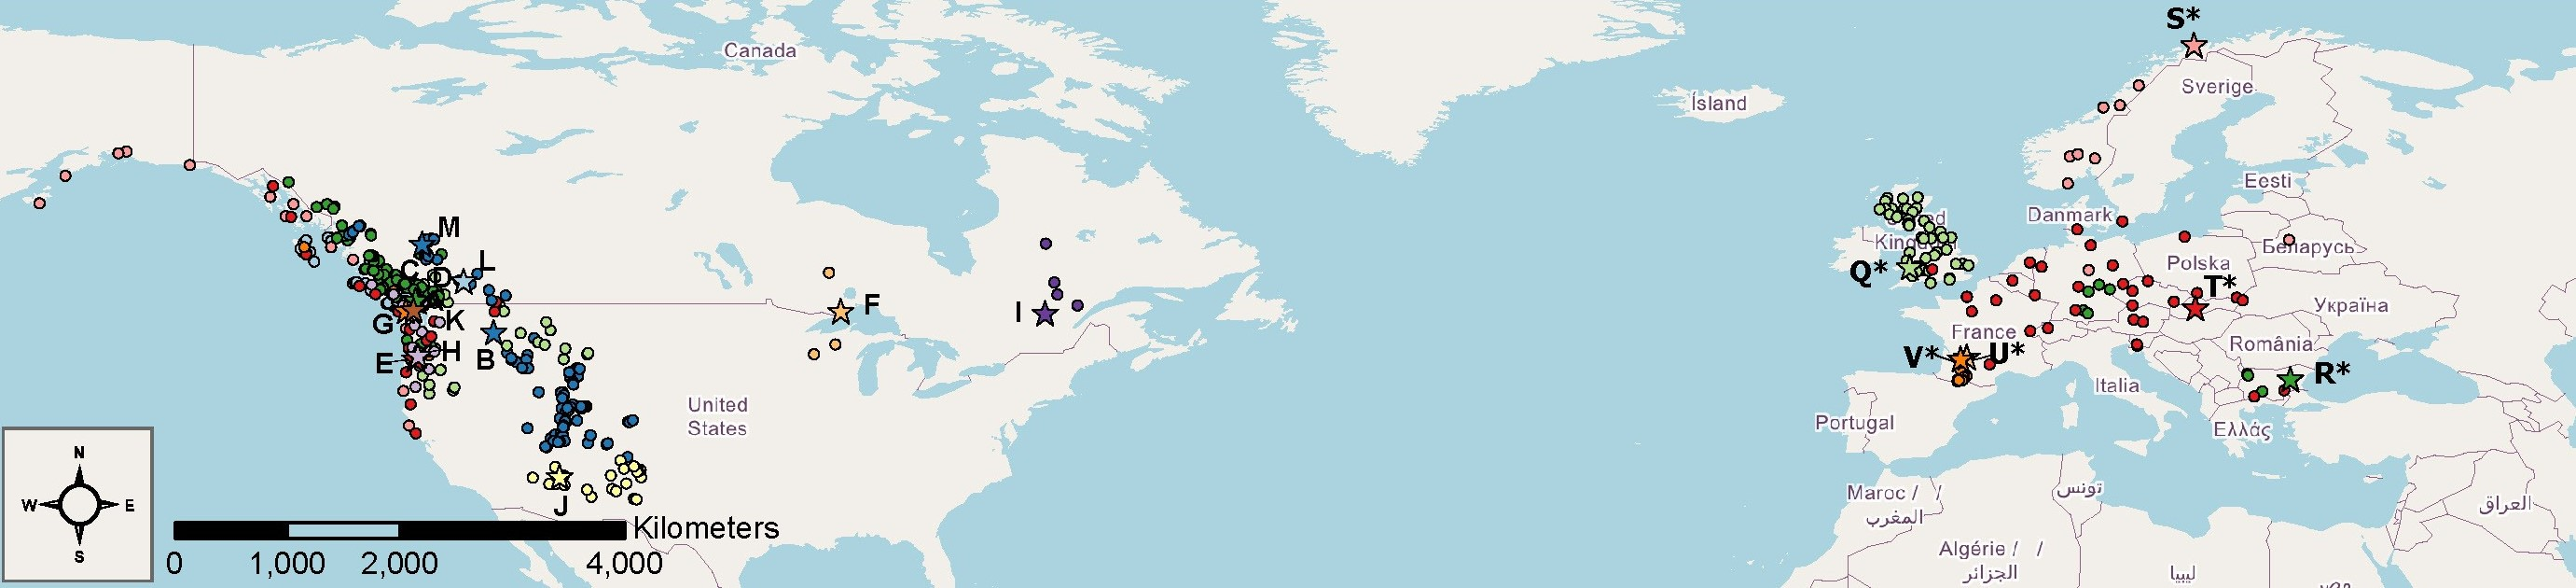
\includegraphics[width=\textwidth]{..//..//localadaptclim/Docs/figure_ms/map_gardens.jpg}
    \caption{Distribution of common gardens (denoted as stars) and provenances (denoted as circles) included in this meta-analysis. The distribution was skewed toward North America (12 North American studies versus 5 European studies). See Table.S\ref{supplement-table:all_studies} in Supporting Information for sourcing information on selected studies. Note: map lines do not necessarily depict accepted national boundaries. European sites are shown in bold and denoted by an asterisk (*). }
    \label{figure:map_gardens}
\end{figure}


\begin{figure}[!h] 
    \centering
 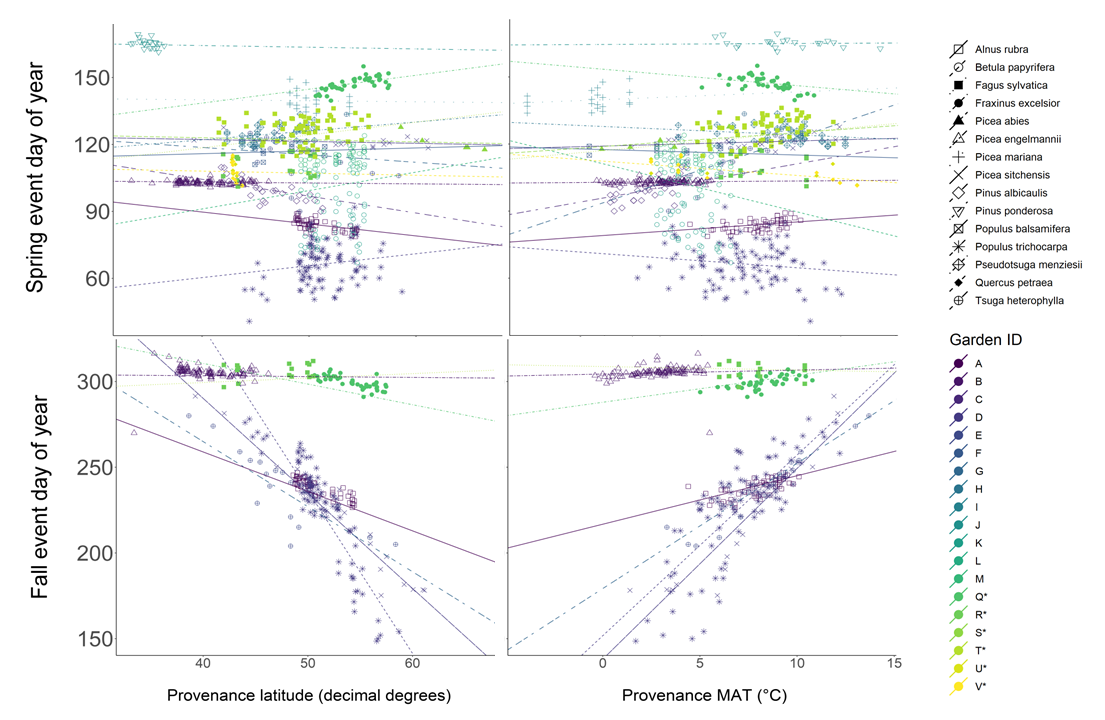
\includegraphics[width=\textwidth]{..//..//localadaptclim/Docs/figure_ms/springfall_latmat.jpg}
    \caption{Event day of year (DOY) in relation to provenance latitude and MAT, coded by symbol for species and color for garden with linear fits from hierarchical Bayesian models. Spring events shown on top and fall events at the bottom. European gardens and species are shown in bold and denoted by an asterisk (*). } 
    \label{figure:springfall_latmat}
\end{figure}

%EMWSep30: Updated figures are nice! I shortened the descriptions in both and re-arranged a little. Try to keep phrasing more consistent here (don't mix 'as we move north' with 'per degree northward' -- pick one). Check my edits closely to make sure they're correct. 
\begin{figure}[!h] 
    \centering
 \includegraphics[width=\textwidth]{..//..//localadaptclim/Docs/figure_ms/continental_spptype_lat.jpg}
    \caption{Effects of latitude on spring and fall event date (DOY) depending on (a \& b) continent, and (c \& d) species leaf type (gymnosperms, which were all evergreen species, versus angiosperms, which were all deciduous species) shown as posterior distributions (full distribution represents 99\% percentile, solid line and shading in posteriors represent mean and 50 percent interval, 90\% intervals given in text). Zero---no effect---is shown with a dashed line.}
    %RM for editor: Spring events did not shift with latitude by continent, but fall events advanced strongly per degree northward, particularly in North America. Spring events slightly advanced in gymnosperms (all evergreen species) and delayed in angiosperms (all deciduous species) per degree northward. Fall events advanced per degree northward for both species types.    
    \label{figure:continental_spptype_lat}
\end{figure}

\begin{figure}[!h] 
    \centering
 \includegraphics[width=\textwidth]{..//..//localadaptclim/Docs/figure_ms/continental_spptype_effect.jpg}
    \caption{Effects of MAT on spring and fall event date (DOY) depending on (a \& b) continent, and (c \& d) species leaf type (gymnosperms, which were all evergreen species, versus angiosperms, which were all deciduous species)  shown as posterior distributions (full distribution represents 99\% percentile, solid line and shading in posteriors represent mean and 50 percent interval, 90\% intervals given in text). Zero---no effect---is shown with a dashed line. } 
    % RM per editor request: Spring events did not shift with MAT by continent, but fall events advanced strongly with decreasing MAT, particularly notably in North America. Spring events slightly advanced in angiosperms and delayed in gymnosperms with increasing MAT. Fall events delayed with increasing MAT for both species types.
    \label{figure:continental_spptype_effect}
\end{figure}






\end{document}







% A data availability statement which provides information about where the research data and other artifacts supporting the results reported in the paper can be found must be submitted. Links to the repository where the dataset(s) are publicly archived and DOIs must be included. A list of standard templates for the text for the ‘Data Availability Statement’ is available here.
% Data must be cited within the text in the in the Materials and Methods section.
% Data must be included as a formal citation in the reference section. More detail on how to do this can be found here.
% Datasets containing population means from all studies are archived in Dryad

% Data Archiving Statement
% Data available from the Dryad Digital Repository: http://dx.doi.org/10.5061/dryad.rj15h


% formatting code resources
% https://github.com/lizzieinvancouver/ospree/blob/master/docs/ranges/ranges_outline.tex
% https://github.com/lizzieinvancouver/ospree/blob/master/docs/traits/Traitors_Manuscript_supp.Rnw

